\documentclass[letterpaper,twocolumn,10pt]{article}

\usepackage[table]{xcolor}
\usepackage{usenix,epsfig}
\usepackage[utf8]{inputenc}
\usepackage{tikz}
\usetikzlibrary{calc}
\usetikzlibrary{positioning}
\usepackage{amsmath}
\usepackage{subfigure}
\usepackage{tabularx}
\usepackage{multirow}
\usepackage{hyperref}
\usepackage{balance}
\usepackage{AlegreyaSans}
\usepackage{xspace}
\usepackage{inconsolata}
\usepackage{balance}
\usepackage[backend=biber,backref=true]{biblatex}
\usepackage[T1]{fontenc}
\usepackage[scaled=0.8]{beramono}
\usepackage{enumitem} % Compact descriptions.

\bibliography{literature}

\renewcommand*{\bibfont}{\footnotesize}

\definecolor{darkblue}{rgb}{0,0,0.4}
\hypersetup{
	pdftitle={Identifying and characterizing Sybils in the Tor network},
	pdfauthor={Philipp Winter, Roya Ensafi, Karsten Loesing, and Nick Feamster},
	colorlinks=true,
	urlcolor=darkblue,
	linkcolor=darkblue,
	citecolor=darkblue
}

\newcommand{\sys}{sybilhunter\xspace}
\newcommand{\Sys}{Sybilhunter\xspace}

\urlstyle{sf}

\newcommand{\mynote}[1]{\noindent\textcolor{red}{\textbf{Note:} #1}}

\begin{document}

\title{\Large \bf Identifying and characterizing Sybils in the Tor network}

\author{
{\rm Philipp Winter}\\
Princeton \& Karlstad \\ University
\and
{\rm Roya Ensafi}\\
Princeton University
\and
{\rm Karsten Loesing}\\
The Tor Project
\and
{\rm Nick Feamster}\\
Princeton University
}

\maketitle

\begin{abstract}
{
Being a volunteer-run, distributed anonymity network, Tor is vulnerable to Sybil
attacks.  Sybil relays can increase exposure to relayed traffic and manipulate
Tor's distributed hash table.  Until now, little was known about real-world
Sybils in the Tor network, and we lack comprehensive tools to find and analyze
Sybil attacks.
%
We develop a system that can detect Sybil relays based on their appearance and
behavior.  Our system can analyze past and future Tor network data for Sybil
attacks.  We discuss the design of our system, and characterize Sybil groups we
discovered.
%
Our work reveals how attackers operate, what they are motivated by, and provides
practical tools to analyze and characterize Tor relays.
}
\end{abstract}


\section{Introduction}
\label{sec:introduction}

% Short introduction to Sybil attacks.
Distributed systems are believed to be more robust than their centralized
counterparts against attacks such as coercion, denial of service, and
surveillance.  The Tor network is no exception. 
However, the absence of a central, controlling authority facilitates
\emph{Sybil attacks}.  Sybil attacks---introduced by Douceur in
2002~\cite{Douceur2002a}---are defined as one physical entity controlling many
virtual identities in a distributed system.  The attack is problematic because
many distributed systems make assumptions on the maximum number of malicious
nodes they can endure.

% How do Sybil attacks relate to Tor? -- DHT manipulation.
An attacker's motivation for performing a Sybil attack differs from system to
system.  In the case of Tor, attackers are frequently motivated by manipulating
Tor's distributed hash table (DHT)~\cite{rendspec}.  We need to take a step back
to show why this is problematic.  Tor clients need a hidden service
descriptor to learn how to connect to a given hidden service such as
\url{3g2upl4pq6kufc4m.onion}, the DuckDuckGo search engine.  These descriptors
are stored in Tor's DHT.  The DHT implementation suffers from a weakness that
allows an attacker to predict at which position in the DHT a descriptor will be
stored.  The attacker can then change its fingerprints to become responsible
for a given hidden service~\cite{Biryukov2013a}.\footnote{This boils down to
brute-forcing the RSA key pair of a relay until its fingerprint is reasonably
close to the descriptor's position in the DHT.}  Six Sybil relays are
sufficient to become the sole responsible party for a hidden service, allowing
the attacker to monitor (still anonymous) clients requests, or refuse to serve
the hidden service, effectively taking it down.

% How do Sybil attacks relate to Tor? -- Increased traffic exposure.
In addition to DHT manipulation, Sybils allow an attacker to increase its
exposure to traffic.  Note that generally, instead of running $n$ relays, an
attacker can run a single relay that provides just as much bandwidth as $n$
relays together.  But at some point, an attacker will have to scale
horizontally because there are limits to how much traffic can be relayed by a
single machine.  Once an attacker can see a non-trivial fraction of Tor
traffic, it is able to:
\begin{description}
	\item[Manipulate exit traffic] to steal passwords, break into TLS
		connections, or inject data~\cite{Winter2014a}.
	\item[End-to-end correlate] traffic by running entry guards as well as exit
		relays~\cite{Johnson2013a}.  Note that a network-level adversary such as
		an ISP or a government might only need to run one of both.
	\item[Harvest bridge addresses] by running middle nodes and isolating the
		IP addresses of incoming Tor connections that don't originate from
		(publicly known) guard relays~\cite{Ling2012a}.
	\item[Website fingerprint] connections on guard relays to learn what
		websites Tor users are connecting to~\cite{Juarez2014a}.
\end{description}

% Sybils can be a side effect.
Instead of being a direct means to an end, Sybils can be a \emph{side effect}
of another issue.  In Section~\ref{sec:sybil_groups}, we provide evidence for
what we believe is a botnet whose members are running Tor relays.  Similarly,
in August 2013, attackers infected computers with malware that used a Tor
hidden service as command and control server~\cite{Hopper2014a}.  In this case,
however, the infected machines were only Tor clients, and not relays.

% Why previously proposed solutions don't work.
Having outlined the problem, it is tempting to look for solutions in the
substantional amount of previous work that proposed Sybil mitigation techniques.
In his seminal 2002 paper~\cite{Douceur2002a}, Douceur formally showed that the
only method guaranteed to keep out Sybils is a \emph{central authority} that
verifies new nodes as they join the distributed system.  This approach conflicts
with Tor's design philosophy because it seeks to eliminate central points of
control.  In addition, a major factor contributing to Tor's growth is the low
barrier of entry, allowing operators to set up relays quickly and anonymously.
A controlling authority would raise that barrier.  Barring a central authority,
researchers have proposed techniques that build on a resource that is difficult
for an attacker to scale.  Past work has focused extensively on
\emph{computational resources} and \emph{edges in social graphs}.

Computational resources can be useful if an attacker that seeks to
operate 100 Sybils suddently needs 100 times the computational resources she
would need for a single virtual identity.  Social graph-based Sybil detection
techniques assume that it is difficult for Sybils to establish a large number of
connections with non-Sybils.  Unfortunately, both resources do not apply to the
Tor network. Requiring relay operators to complete proof-of-works is pointless
as running a relay already involves computational work.  Social graph-based
defenses do not apply because there is no trust relationship between Tor
relays.\footnote{To clarify, relay operators are encouraged to set the
\texttt{MyFamily} option for relays under their control, but this type of
trust relationship does not span to relays run by others.}

% Our contributions.
Given the nonapplicability of existing approaches, we focus on techniques to
find Sybils in the Tor network.  We implemented these techniques in a tool,
sybilhunter, which we then use to analyze historical network data, dating back
to as early as 2007, to discover past attacks and anomalies.  Finally, we
extensively characterize the Sybil groups we discover.  To sum up, we provide
the following contributions:
\begin{itemize}
	\item We consider Sybils in Tor and show how this problem differs from
		related work.
	\item Design and implement a platform for continuous monitoring of archived
		Tor data.
	\item Analze past incidents in-depth and publish dataset for future
		research.
\end{itemize}

% Structure of the paper.
The rest of this paper is structured as follows.  We begin by discussing
related work in Section~\ref{sec:related_work}.  Section~\ref{sec:design}
presents the design of our analysis tools, which is then followed by
experimental results in Section~\ref{sec:results}.  We discuss our results in
Section~\ref{sec:discussion} and conclude the paper in
Section~\ref{sec:conclusion}.


\section{Related work}
\label{sec:related_work}
% Why previously proposed solutions don't work.
In his seminal 2002 paper, Douceur showed that only a \emph{central authority}
that verifies new nodes as they join the distributed system is guaranteed to
prevent Sybils~\cite{Douceur2002a}.  This approach conflicts with Tor's design
philosophy that seeks to eliminate central points of control and distribute
trust.  In addition, a major factor contributing to Tor's relay growth is the
low barrier of entry, allowing operators to set up relays quickly and
anonymously.  An identity-verifying authority would raise that barrier, alienate
privacy-conscious relay operators, and impede Tor's growth.  Barring a central
authority, researchers have proposed techniques that leverage a resource that is
difficult for an attacker to scale.  Two categories of Sybil-resistant schemes
turned out to be particularly popular, schemes that build on \emph{social
constraints} and schemes that build on \emph{computational constraints}.  For a
broad overview of alternative Sybil defenses, refer to Levine et
al.~\cite{Levine2006a}.

Social constraints rely on the assumption that it is difficult for an attacker
to form trust relationships with honest users, e.g., befriend many unknown
people on online social networks.  Past work leveraged this assumption in
systems such as SybilGuard~\cite{Yu2006a}, SybilLimit~\cite{Yu2008a}, and
SybilInfer~\cite{Danezis2009a}.  Unfortunately, social graph-based defenses
do not work in our setting because there is no existing trust relationship
between relay operators.\footnote{Relay operators can express in their
configuration that their relays are run by the same operator, using the
\texttt{MyFamily} option, but this denotes an \emph{intra}-person and not an
\emph{inter}-person trust relationship.} Note that we could create such a
relationship by, e.g., linking relays to their operator's social networking
account, or by creating a ``relay operator web of trust,'' but again, we
believe that such an effort would alienate relay operators and receive limited
adoption.

Orthogonal to social constraints, computational resource constraints guarantee
that an attacker that seeks to operate 100 Sybils needs 100 times the
computational resources she would have needed for a single virtual identity.
Both Borisov~\cite{Borisov2006a} and Li et al.~\cite{Li2012a} used computational
puzzles for that purpose.  Computational constraints work well in distributed
systems where the cost of joining the network is low.  For example, to use
BitTorrent, a user only needs to run a lightweight client.  However, this is not
the case in Tor because relay operations require constant use of bandwidth and
CPU.  Unlike in many other distributed systems, it is impossible to run 100 Tor
relays while not spending the resources for 100 relays.  In a way, computational
constraints are inherent to running a relay.

In summary, we believe that existing Sybil defences do not work well when
applied to the Tor network; its destinctive features call for special solutions.


\section{Background}
\label{sec:background}
We now provide necessary background on the Tor network~\cite{Dingledine2004a}.
Tor consists of several thousand volunteer-run relays that are summarized in the
\emph{network consensus} that is voted on and published every hour by eight
distributed \emph{directory authorities}.  The authorities assign a variety of
flags to relays:

\begin{description}
	\item[Valid:] The relay is valid, i.e., not known to be broken.
	\item[HSDir:] The relay is an onion service directory, i.e., it participates
		in the DHT that powers Tor onion services.
	\item[Exit:] The relay is an exit relay.
	\item[BadExit:] The relay is an exit relay but is either misconfigured or
		malicious, and should therefore not be used by Tor clients.
	\item[Stable:] Relays are stable if their mean time between failure is at
		least the median of all relays, or at least seven days.
	\item[Guard:] Guard relays are the rarely-changing first hop for Tor clients.
	\item[Running:] A relay is running if the directory authorities could
		connect to it in the last 45 minutes.
\end{description}

Tor relays are uniquely identified by their \emph{fingerprint}, a Base32-encoded
and truncated SHA-1 hash over their public key.  Operators can further assign a
\emph{nickname} to their Tor relays, which is a string that identifies a relay
(albeit not uniquely) and is easier to remember than its pseudo-random
fingerprint.  Exit relays have an \emph{exit policy}---a list of IP addresses
and ports that the relay allows connections to.  Finally, operators that run
more than one relay are encouraged to configure their relays to be part of a
\emph{relay family}.  Families are used to express that a set of relays is
controlled by a single party.  Tor clients never use more than one family member
in their path to prevent correlation attacks.


\section{Data and design}
\label{sec:design}
We define Sybils in the Tor network as two or more relays that are controlled by
a single person or group of people.  Sybils per se do not have to be malicious;
a relay operator could simply have forgotten to configure her relays as a relay
family.  Such Sybils are no threat to the Tor network, which is why we refer to
them as \emph{benign Sybils}.  What we are interested in is \emph{malicious
Sybils} whose purpose is to deanonymize or otherwise harm Tor users.

We draw on two datasets---one publicly available and one created by us---to
uncover malicious Sybils.  Our detection methods are implemented in a tool,
\sys, which takes as input our two datasets and then attempts to expose Sybil
groups, as illustrated in Figure~\ref{fig:system}.  \Sys is implemented in Go
and consists of 3,300 lines of code.

\begin{figure}[t]
	\centering
	\includegraphics[width=0.8\linewidth]{diagrams/architecture.pdf}
	\caption{\Sys's architecture.  Two datasets serve as input to
		\sys; consensuses and server descriptors, and malicious
		relays gathered with exitmap~\cite{Winter2014a}.}
	\label{fig:system}
\end{figure}

\subsection{Datasets}
\label{sec:datasets}
Figure~\ref{fig:system} shows how we use our two datasets.  Archived consensuses
and router descriptors (in short: descriptors) allow us to (\emph{i}) restore
past states of the Tor network, which \sys mines for Sybil groups, and to
(\emph{ii}) find ``partners in crime'' of malicious exit relays that we
discovered by running exitmap, a scanner for Tor exit relays that is presented
below.

\subsubsection{Consensuses and router descriptors}
The consensus and descriptor dataset is publicly available on
CollecTor~\cite{collector}, an archiving service that is run by The Tor Project.
Some of the archived data dates back to 2004, allowing us to restore arbitrary
Tor network configurations from the last ten years.  Not all of CollecTor's
archived data is relevant to our hunt for Sybils, however, which is why we only
analyze the following two:

\begin{figure}[t]
\centering
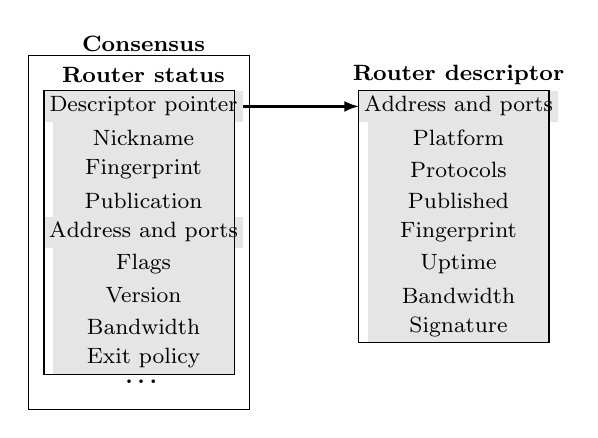
\begin{tikzpicture}[node distance=0 cm,outer sep = 0pt,inner sep = 2pt]

	\tikzstyle{every node}=[font=\footnotesize]

	\tikzset{field/.style={align=center,shape=rectangle,
		minimum height=4mm,minimum width=23mm,fill=gray!20}}

	\tikzset{blankfield/.style={align=center,shape=rectangle,
		minimum height=4mm,minimum width=23mm}}

	\usetikzlibrary{positioning}

	\node (consensus) [blankfield] {\textbf{Consensus}};

	% Router status fields, one below another.
	\node (routerstatus) [blankfield,below=of consensus] {\textbf{Router status}};
	\node (desc) [field,below=of routerstatus] {Descriptor pointer};
	\node (nickname) [field,below=of desc] {Nickname};
	\node (fingerprint) [field,below=of nickname] {Fingerprint};
	\node (publication) [field,below=of fingerprint] {Publication};
	\node (address) [field,below=of publication] {Address and ports};
	\node (flags) [field,below=of address] {Flags};
	\node (version) [field,below=of flags] {Version};
	\node (bandwidth) [field,below=of version] {Bandwidth};
	\node (policy) [field,below=of bandwidth] {Exit policy};
	\node [below=of policy] {\textbf{\dots}};

	% Draw a rectangle around a router status.
	\draw [draw=black] (desc.north west) rectangle (policy.south east);

	% Draw a rectangle around multiple router statuses.
	\draw [draw=black] ($(desc.north west) + (-2mm,4.5mm)$) rectangle ($(policy.south east) + (2mm,-4.5mm)$);

	% Router descriptor fields, one below another.
	\node (dummy) at (4cm,0) [blankfield] {};
	\node (descriptor) at (4cm,0) [blankfield,below=of dummy] {\textbf{Router descriptor}};
	\node (descaddr) at (4cm,0) [field,below=of descriptor] {Address and ports};
	\node (descplatform) at (4cm,0) [field,below=of descaddr] {Platform};
	\node (descprotocols) at (4cm,0) [field,below=of descplatform] {Protocols};
	\node (descpublished) at (4cm,0) [field,below=of descprotocols] {Published};
	\node (descfingerprint) at (4cm,0) [field,below=of descpublished] {Fingerprint};
	\node (descuptime) at (4cm,0) [field,below=of descfingerprint] {Uptime};
	\node (descbandwidth) at (4cm,0) [field,below=of descuptime] {Bandwidth};
	\node (descsignature) at (4cm,0) [field,below=of descbandwidth] {Signature};

	% Draw a rectangle around a descriptor.
	\draw [draw=black] (descaddr.north west) rectangle (descsignature.south east);

	% Pointer from digest to descriptor.
	\draw [-latex,thick] (desc) -- (descaddr);
\end{tikzpicture}
\caption{Our primary dataset contains consensuses and router descriptors.}
\label{fig:datasets}
\end{figure}

\paragraph{Descriptors} Tor relays and bridges periodically upload router
descriptors, which capture their configuration, to directory authorities.
Figure~\ref{fig:datasets} shows an example in the box to the right.  Relays
upload their descriptors no later than every 18 hours, or sooner, depending on
certain conditions.  Note that some information in router descriptors is not
verified by directory authorities.  Therefore, relays can spoof information such
as their operating system, Tor version, and uptime.

\paragraph{Consensuses} Each hour, the nine directory authorities vote on their
view of all Tor relays that are currently online.  The vote produces the
consensus, an authoritative list that comprises all running Tor relays,
represented as a set of router statuses.  Each router status in the consensus
contains basic information about Tor relays such as their bandwidth, flags, and
exit policy.  It also contains a pointer to the relay's descriptor, as shown in
Figure~\ref{fig:datasets}.  As of February 2016, consensuses contain
approximately 7,000 router statuses, i.e., each hour, 7,000 router statuses are
published, and archived, by CollecTor.

Table~\ref{tab:collector-dataset} gives an overview of the size of our consensus
and descriptor archives.  We found it challenging to repeatedly process these
millions of files, amounting to more than 100 GiB of uncompressed data.  In our
first processing attempt, we used the Python parsing library Stem~\cite{stem},
which is maintained by The Tor Project.  The data volume turned out to be
difficult to handle for Stem because of Python's interpreted and dynamic nature.
To process our dataset more efficiently, we implemented a custom parser in
Go~\cite{zoossh}.

\begin{table}[t]
\small
\centering
\begin{tabular}{l r r r}
\toprule
\textbf{Dataset} & \textbf{\# of files} & \textbf{Size} & \textbf{Time span} \\
\midrule
% find . -type f | wc -l
% du -b consensuses/
Consensuses & 72,061 & 51 GiB & 10/2007--01/2016 \\
Descriptors & 34,789,777 & 52 GiB & 12/2005--01/2016 \\
\bottomrule
\end{tabular}
\caption{An overview of our primary dataset; consensuses and server descriptors
since 2007 and 2005, respectively.}
\label{tab:collector-dataset}
\end{table}

\subsubsection{Malicious exit relays}
In addition to our publicly available and primary dataset, we collected
malicious exit relays over 18 months.  We call exit relays malicious if they
modify forwarded traffic in bad faith, e.g., to run man-in-the-middle attacks.
We add these relays to our dataset because they frequently \emph{surface in
groups}, as malicious Sybils, because an attacker runs the same attack on
several, physically distinct exit relays.  Winter et al.'s
work~\cite[\S~5.2]{Winter2014a} further showed that attackers make an effort to
stay under the radar, which is why we cannot only rely on active probing to
find such relays.  We also seek to find potential ``partners in crime'' of each
newly discovered malicious relay, which we discuss in
Section~\ref{sec:nearest-neighbor}.

We exposed malicious exit relays using Winter et al.'s exitmap
tool~\cite{Winter2014a}.  Exitmap is a Python-based scanning framework for Tor
exit relays.  Exitmap modules perform a network task that can then be run over
all exit relays.  One use case is HTTPS man-in-the-middle detection: A module
can fetch the certificate of a web server over all exit relays and then compare
its fingerprint with the expected, valid fingerprint.  Exposed attacks are
sometimes difficult to attribute because an attack can take place upstream of the
exit relay, e.g., at a malicious autonomous system.  However, attribution is
only a secondary concern.  Our primary concern is protecting Tor users from
harm, and we do not need to identify the culprit to succeed.

In addition to the original modules that the exitmap authors shared with us, we
implemented exitmap modules to detect HTML tampering and TLS downgrading, by
connecting to servers under our control and raising an alert if the returned
HTML or TLS server hello were modified.  Our modules ran from August 2014 to
January 2016 and discovered 251 malicious exit relays whose attacks are
discussed in Appendix~\ref{sec:malicious-relays}.  We reported all relays to The
Tor Project, which subsequently blocked these relays.

\subsection{Threat model}
\label{sec:threat_model}
Most of this paper is on applying \sys to archived network data, but we can also
apply it to newly incoming data.  This puts us in an adversarial setting as
attackers can tune their Sybils to evade our system.  This is reflected in our
adversarial assumptions.  We assume that an adversary \emph{does} run more than
one Tor relay and exhibits redundancy in their relay configuration, or uptime
sequence.  An adversary further \emph{can} know how \sys's modules work, run
active or passive attacks, and make a limited effort to stay under the radar, by
diversifying parts of their configuration.  To detect Sybils, however, our
heuristics require \emph{some} redundancy.

\subsection{Analysis techniques}
\label{sec:techniques}
Having discussed our datasets and threat model, we now turn to presenting
techniques that can expose Sybils.  Our techniques are based on the insight that
Sybil relays typically \emph{behave or appear similarly}.  Shared configuration
parameters such as port numbers and nicknames cause similar appearance whereas
Sybils behave similarly when they reboot simultaneously, or exhibit identical
quirks when relaying traffic.

\Sys can analyze (\emph{i}) historical network data, dating back to 2007;
(\emph{ii}) online data, to detect new Sybils as they join the network; and
(\emph{iii}) find relays that might be associated with previously discovered,
malicious relays.  Figure~\ref{fig:shr-internal} shows \sys's internal
architecture.  Tor network data first passes a filtering component that can be
used to inspect a subset of the data, e.g., only relays with a given IP address
or nickname.  The data is then forwarded to one or more modules that implement
an analysis technique.  These modules work independently, but share a data
structure to find suspicious relays that show up in more than one module.
Depending on the analysis technique, \sys's output is CSV files or images.

\begin{figure}[t]
	\centering
	\includegraphics[width=0.9\linewidth]{diagrams/internal-architecture.pdf}
	\caption{\Sys's internal architecture.}
	\label{fig:shr-internal}
\end{figure}

While developing \sys, we had to make many design decisions that we
tackled by drawing on the experience we gained by manually analyzing numerous
Sybil groups.  We iteratively improved our code and augmented it with new
features when we experienced operational shortcomings.

\subsubsection{Network churn}
\label{sec:churn-time-series}
The churn rate of a distributed system captures the rate of joining and leaving
network participants.  In the Tor network, these participants are relays.  An
unexpectedly high churn rate between two subsequent consensuses means that many
relays joined or left, which can reveal Sybils and other network issues because
Sybil operators frequently start and stop their Sybils at the same time, to ease
administration---they behave similarly.

The Tor Project is maintaining a Python script~\cite{doctor} that determines the
number of previously unobserved relay fingerprints in new consensuses.  If that
number is greater than or equal to the static threshold 50, the script sends an
e-mail alert.  We reimplemented the script in \sys and ran it over all archived
consensus documents, dating back to 2007.  The script raised 47 alerts in nine
years, all of which seemed to be true positives, i.e., they should be of
interest to The Tor Project.  The script did not raise false positives,
presumably because the median number of new fingerprints in a consensus is only
six---significantly below the conservative threshold of 50.  Yet, the threshold
likely causes false negatives, but we cannot determine the false negative rate
because we lack ground truth.  In addition, The Tor Project's script does not
consider relays that left the network, does not distinguish between relays with
different flags, and does not adapt its threshold as the network grows.  We now
present an alternative approach that is more flexible and robust.

We found that churn anomalies worthy of our attention range from \emph{flat
hills} (Fig.~\ref{fig:flat-hill}) to \emph{sudden spikes}
(Fig.~\ref{fig:sudden-spike}).  Flat hills can be a sign of an event that
concerned a large number of relays, over many hours or days.  Such an event
happened shortly after the Heartbleed bug, when The Tor Project asked relay
operators to generate new keys.  Relay operators acted gradually, most within
two days.  Sudden spikes can happen if an attacker adds many relays, all at
once.  These are mere examples, however; the shape of a time series cannot tell
us anything about the nature of the underlying incident.

\begin{figure}[t]
	\centering
	\includegraphics[width=\linewidth]{diagrams/flat-hill.pdf}
	\caption{A flat hill of new relays in 2009.  The time series was smoothed
	using a moving average with a window size of 12 hours.}
	\label{fig:flat-hill}
\end{figure}

\begin{figure}[t]
	\centering
	\includegraphics[width=\linewidth]{diagrams/sudden-spike.pdf}
	\caption{A sudden spike of new relays in 2010.  The time series was smoothed
	using a moving average with a window size of 12 hours.}
	\label{fig:sudden-spike}
\end{figure}

To quantify the churn rate $\alpha$ between two subsequent consensus documents,
we adapt Godfrey et al.'s formula, which yields a churn value that captures
both systems that joined and systems that left the
network~\cite[\S~2.1]{Godfrey2006a}.  However, an unusually low number of
systems that left could cancel out an unusually high number of new systems and
vice versa---an undesired property for a technique that should spot abnormal
changes.  To address this issue, we split the formula in two parts, creating a
time series for new relays ($\alpha_{n}$) and for relays that left
($\alpha_{l}$).  $C_{t}$ is the network consensus at time $t$, and $\setminus$
denotes the complement between two consensuses, i.e., the relays that are in
the left operand, but not the right operand.  We define $\alpha_{n}$ and
$\alpha_{l}$ as

\begin{equation}
\alpha_{n} = \frac{\lvert C_{t} \setminus C_{t-1} \rvert}
{\lvert C_{t} \rvert}
\qquad\text{and}\qquad
\alpha_{l} = \frac{\lvert C_{t-1} \setminus C_{t} \rvert}
{\lvert C_{t-1} \rvert}.
\end{equation}

Both $\alpha_{n}$ and $\alpha_{l}$ are bounded to the interval $[0, 1]$.  A
churn value of 0 indicates no change between two subsequent consensuses whereas
a churn value of 1 indicates a complete turnover.  Determining $\alpha_{n,l}$
for the sequence $C_{t}, C_{t-1}$, \ldots, $C_{t-n}$, yields a time series of
churn values that can readily be inspected for abnormal spikes.  We found that
many churn anomalies are caused by relays that share a flag, or a flag
combination, e.g., \texttt{HSDir} (onion service directories) and \texttt{Exit}
(exit relays).  Therefore, \sys can also generate per-flag churn time series
that can uncover patterns that would be lost in a flag-agnostic time series.

Finally, to detect changes in the underlying time series trend---flat hills---we
can smooth $\alpha_{n,l}$ using a simple moving average $\lambda$ defined as

\begin{equation}
\lambda = \frac{1}{w} \cdot \sum_{i=0}^{w} \alpha_{i}.
\end{equation}

As we increase the window size $w$, we can detect more subtle changes in the
underlying churn trend.  If $\lambda$ or $\alpha_{n,l}$ exceed a manually
defined threshold, an alert is raised.  Section~\ref{sec:churn} elaborates on
how a threshold can be chosen in practice.

\subsubsection{Uptime matrix}
\label{sec:uptime-matrix}
For convenience, Sybil operators are likely to administer their relays
simultaneously, i.e., update, configure, and reboot them all at the same time.
This is reflected in their relays' uptime.  An operating system upgrade that
requires a reboot of Sybil relays will induce a set of relays to go offline and
return online in a synchronized manner.  To isolate such events, we are
visualizing the \emph{uptime patterns} of Tor relays by grouping together relays
whose uptime is highly correlated.  The churn technique presented above is
similar but it only provides an aggregate, high-level view on how Tor relays
join and leave the network.  Since the technique is aggregate, it is poorly
suited for visualizing the uptime of specific relays; an abnormally high churn
value attracts our attention but does not tell us what caused the anomaly.  To
fill this gap, we complement the churn analysis with an uptime matrix that we
will now present.

This uptime matrix consists of the uptime patterns of all Tor relays, which we
represent as binary sequences.  Each hour, when a new consensus is published, we
add a new data point---``online'' or ``offline''---to each Tor relay's sequence.
We visualize all sequences in a bitmap whose rows represent consensuses and
whose columns represent relays.  Each pixel denotes the uptime status of a
particular relay at a particular hour.  Black pixels mean that the relay was
online and white pixels mean that the relay was offline.  This type of
visualization was first proposed by Ensafi and subsequently implemented by
Fifield~\cite{Fifield2014a}.

Of particular importance is how the uptime sequences are sorted.  If highly
correlated sequences are not adjacent in the visualization, we might miss them.
We sort sequences using single-linkage clustering, a type of hierarchical
clustering algorithm that forms groups bottom-up, based on the minimum distance
between group members.  Our clustering algorithm requires a distance function.
Similar to Andersen et al.~\cite[\S~II.B]{Andersen2002a}, we use Pearson's
correlation coefficient as our distance function because it tells us if two
uptime sequences change together.  The sample correlation coefficient $r$
yields a value in the interval $[-1, 1]$.  A coefficient of $-1$ denotes
perfect anti-correlation (relay $R_1$ is only online when relay $R_2$ is
offline) and 1 denotes perfect correlation (relay $R_1$ is only online when
relay $R_2$ is online).  We define our distance function as $d(r) = 1 - r$, so
two perfectly correlated sequences have a distance of zero while two perfectly
anti-correlated sequences have a distance of two.  Once all sequences are
sorted, we color adjacent sequences in red if their uptime sequence is
identical.  Figure~\ref{fig:uptime-matrix} shows an example of our
visualization algorithm, the uptime matrix for a subset of all Tor relays in
November 2012.

\begin{figure}[t]
	\centering
	\includegraphics[width=\linewidth]{diagrams/2012-11.jpg}
	\caption{The uptime matrix for 3,000 Tor relays for all of November 2012.
	Rows represent consensuses and columns represent relays.  Black pixels mean
	that a relay was online, and white means offline.  Red blocks denote relays
	with identical uptime.}
	\label{fig:uptime-matrix}
\end{figure}

\subsubsection{Fingerprint analysis}
\label{sec:fingerprint-analysis}
The information a Tor client needs to connect to an onion service is stored in a
DHT that consists of a subset of all Tor relays, the onion service directories
(HSDirs).  As of February 2016, 46\% of all Tor relays serve as HSDirs.  A
daily-changing set of six HSDirs host the contact information of any given
onion service.  Tor clients contact one of these six HSDirs to request
information about the onion service they intend to connect to.  A HSDir becomes
responsible for an onion service if the difference between its relay fingerprint
and the service's descriptor ID is smaller than that of any other relay.  The
descriptor ID is derived from the onion service's public key, a time stamp, and
additional information.
% https://gitweb.torproject.org/torspec.git/tree/rend-spec.txt:231
% descriptor-id = H(permanent-id | H(time-period | descriptor-cookie | replica))
All HSDirs are public, making it possible to determine at which position in the
DHT an onion service will end up at any point in the future.  Attackers can
exploit the ability to predict the DHT position by repeatedly generating
identity keys until their fingerprint is sufficiently close to the targeted
onion service's index, thus becoming its HSDir~\cite[\S~V.A]{Biryukov2013a}.

We detect relays that change their fingerprint frequently by maintaining a
lookup table that maps a relay's IP address to a list of all fingerprints we
have seen it use.  We sort the lookup table by the relays that changed their
fingerprints the most, and output the results.

\subsubsection{Nearest-neighbor search}
\label{sec:nearest-neighbor}
We frequently found ourselves in a situation where exitmap discovered a
malicious exit relay and we were left wondering if there were similar,
potentially associated relays.  Looking for such relays involved extensive
manual work, which we soon started to automate.  We needed an algorithm for
nearest-neighbor search that takes as input a ``seed'' relay and finds its $n$
most similar neighbors.  We define similarity as shared configuration
parameters such as port numbers, IP addresses, exit policies, or bandwidth
values.  Our search algorithm sorts relays by comparing these configuration
parameters.

To quantify the similarity between two relays, we use the Levenshtein distance,
a distance metric that takes as input two strings and determines the minimum
number of modifications---insert, delete, and modify---that are necessary to
turn string $s_{2}$ into $s_{1}$.  Our algorithm turns the router statuses and
descriptors of two relays into strings and determines their Levenshtein
distance.  As an example, consider a simplified configuration representation
consisting of the concatenation of nickname, IP address, and port.  To turn
string $s_2$ into $s_1$, six operations are necessary; four modifications
(green) and two deletions (red):

\definecolor{change}{rgb}{0.7,1.0,0.7}
\definecolor{delete}{rgb}{1.0,0.7,0.7}

$s_1$: \texttt{Foo10.0.0.19001}

$s_2$: \texttt{\setlength{\fboxsep}{0pt}%
\colorbox{change}{\strut Bar}10.0.0.%
\colorbox{change}{\strut 2}%
\colorbox{delete}{\strut 54}%
9001}

Our algorithm determines the Levenshtein distance between a ``seed'' relay and
all $n-1$ relays in a consensus.  It then sorts the calculated distances in
ascending order and prints the most similar relays.  For a consensus consisting
of 6,525 relays, our algorithm takes approximately 1.5 seconds to
finish.\footnote{We measured on an Intel Core i7-3520M CPU at 2.9 GHz, a
consumer-grade CPU.} Note that we designed nearest-neighbour to assist in
manual analysis.  Unlike the other analysis techniques, it does not require a
threshold.


\section{Evaluation and results}
\label{sec:results}
We now discuss the results we obtained by applying our techniques on our
datasets, nine years worth of archived data.  We begin by presenting the results
of the churn rate analysis, followed by the uptime analysis, and the fingerprint
analysis.  Next, we characterize the most interesting Sybils we found in our
analysis.  Finally, we evaluate our nearest-neighbor search and the
computational performance of all our analysis techniques.

Once we discovered a seemingly harmful Sybil group, we reported it to The Tor
Project.  There are currently two ways for directory authorities to remove
relays, controlled by the options \texttt{AuthDirReject} and
\texttt{AuthDirInvalid}.  The former removes a relay from the consensus and the
latter takes away a relay's \texttt{Valid} flag.  While the relay is still
listed in the consensus, clients will not consider it for their first or last
hop in a circuit.

The majority of directory authorities, i.e., five out of eight, must agree on
either \texttt{AuthDirReject} or \texttt{AuthDirInvalid} to be set for a relay.
Only then will the block become active.  This mechanism is meant to distribute
the power of removing relays into the hands of a diverse set of people.

\subsection{Sybil characterization}
\label{sec:sybil_groups}
Table~\ref{tab:sybils} contains the Sybil groups we identified using our
sybilhunter heuristics and our custom exitmap modules.  For every group, we
document when we first discovered it, its ``name,'' maximal size, and a
description of its purpose.  We now give an overview of the more interesting
groups we exposed.

\begin{table*}[t]
\small
\centering
\begin{tabularx}{\textwidth}{c|c c c c X}
\textbf{Purpose} & \textbf{First active} & \textbf{Group ID} & \textbf{\# of
relays} & \textbf{Heuristic} & \textbf{Description} \\
\hline
%2015-11-28 & foo & 60 & not sure. \\

\multirow{6}{*}{MitM}
& 2015-11 & rewrite$\dagger$ & 8 & EM & Replaced onion domains with impersonation
site. \\

& 2015-06 & rewrite$\dagger$ & 55 & EM & Replaced onion domains with impersonation
site. \\

& 2015-04 & rewrite$\dagger$ & 70 & EM & Replaced onion domains with impersonation
site. \\

& 2015-03 & redirect$\ddagger$ & 24 & EM & Redirected users to impersonated site.
\\

& 2015-02 & redirect$\ddagger$ & 17 & EM & Redirected users to impersonated site.
\\

& 2015-01 & redirect$\ddagger$ & 23 & EM & Redirected users to impersonated site.
\\

\hline

\multirow{3}{*}{DHT}
& 2015-06 & fingerprints & 28 & FPR & All relays, located in the same /24, changed
their fingerprint regularly, presumably in an attempt to manipulate the
distributed hash table. \\

& 2014-01 & FDCservers & 126 & UP & Relays that were involved in an onion service
deanonymization attack~\cite{cmucert}. \\

\hline

\multirow{2}{*}{Botnet}
& 2015-08 & default & --- & F & Likely a Windows-powered botnet.  The group features
wide, geographical distribution, which is uncommon for typical Tor relays. \\

& 2010-09 & trotsky & 219 & F & The relays could have been part of a botnet. \\

\hline

\multirow{5}{*}{Unknown}
& 2015-10 & 11BX1371 & 142 & F & All relays were in two /24 networks and a single
relay had the \texttt{Exit} flag.  \\

& 2015-07 & DenkoNet & 58 & F & Hosted on Amazon AWS and only present in a single
consensus.  No relay had the \texttt{Exit} flag. \\

& 2015-07 & cloudvps & 55 & F & All relays only had the \texttt{Running} and
\texttt{Valid} flag.  As their name suggests, the relays were hosted by the
Dutch hoster ``CloudVPS.'' \\

% Shared: nickname, IP address, port, platform, version.
& 2014-12 & Anonpoke & 284 & F & The relays did not have the \texttt{Exit} flag
and were removed from the network before they could get the \texttt{HSDir} flag.
\\

& 2014-12 & FuslVZTOR & 246 & F & The relays showed up only hours after the
LizardNSA incident. \\

\hline

\multirow{1}{*}{DoS}
& 2014-12 & LizardNSA & 3,347 & UP,CRN & A group publicly claimed to be responsible
for the attack~\cite{lizards}.  All relays were hosted in the Google cloud and
The Tor Project removed them within hours. \\

\hline

\multirow{2}{*}{Research}
& 2010-06 & planetlab & 512 & UP & According to a report from The Tor
Project~\cite{progressreport}, a researcher started these relays to learn more
about scalability effects. \\

& 2013-02 & AmazonEC2 & 57 & FPR & The relays were likely part of a research
project~\cite{Biryukov2013a}. \\

\end{tabularx}
\caption{The Sybil groups we discovered using sybilhunter and our custom exitmap
modules, grouped by their purpose.  We believe that groups marked with the
symbols $\dagger$ and $\ddagger$ were run by the same operator, respectively.}
\label{tab:sybils}
\end{table*}

\paragraph{The ``rewrite'' Sybils}
All relays had the \texttt{Exit} flag and replaced onion domains in HTTP page
fetches with an impersonation, presumably hosted by the attacker.
Interestingly, the impersonation domains shared a prefix with the original,
e.g., \textbf{sigaint}evyh2rzvw.onion was replaced with
\textbf{sigaint}z7qjj3val.onion.  The shared prefix means that the attacker was
generating vanity domains by repeatedly generating public key pairs until the
hash over the key resembled the desired prefix.  Onion domains are generated by
determining the SHA-1 hash over the public key, truncating it to the 80 most
significant bits, and encoding it in Base32.  Each Base32 digit of the
16-digit-domain represents five bits.  As a result, to get an $n$-digit prefix
in the onion domain, $2^{5 n - 1}$ operations are required on average.  For the
seven-digit prefix above, this results in $2^{5 \cdot 7 - 1} = 2^{34}$
operations.  The author of scallion~\cite{scallion}, a tool for generating
vanity onion domains, determined that an nVidia Quadro K2000M, a mid-range
laptop GPU, is able to generate 90 million hashes per second.  On this GPU, a
partial collision for a seven-digit prefix can be found in $2^{34} \cdot
\frac{1}{90,000,000} \simeq 190$ seconds, i.e., in a little bit more than three
minutes.

We found that attacked onion domains contained Bitcoin wallet addresses that
were replaced in the impersonation, presumably to hijack donations or payments.
As a result, we believe that the attack was financially motivated.

\paragraph{The ``redirect'' Sybils}
The relays all had the \texttt{Exit} flag and tampered with HTTP redirects of
exit traffic.  Some Bitcoin sites would redirect users from their HTTP version
to the secure HTTPS version, to protect their users' login credentials.  This
Sybil group, however, tampered with the redirect and directed users towards an
impersonation site, resembling the original Bitcoin site, perhaps to steal
credentials.  We only observed this attack for Bitcoin sites, but cannot rule
out that other sites were not attacked.

Interestingly, the Sybils' server descriptors and consensus entries had less in
common than other Sybil groups.  They used a small set of different ports, Tor
versions, bandwidth values, and their nicknames did not exhibit an
easily-recognizable pattern.  In fact, we can only clearly identify these Sybils
because of the active attack they run, using exitmap, and not because of their
appearance.

We discovered three Sybil groups that implemented the redirect attack, each of
them surfacing when the previous one got blocked.  The first group first showed
up in May 2014, with only two relays, but slowly grew over time, until it was
finally discovered in Jan 2015.  We believe that they were run by the same
attacker because of the way the attack was implemented.

\paragraph{The ``default'' Sybils}
This Sybil group, named after the shared nickname ``default,'' has been around
since 2011 (see Figure~\ref{fig:default-over-time}) and consists of
Windows-powered relays only.  We extracted relays by filtering consensuses
for nicknames that are set to ``default,'' onion routing ports set to 443, and
directory ports set to 9030.  The group features high IP address churn.  For
Oct. 2015, we found ``default'' relays in 73 countries, with the top three
countries being Germany~(50\%), Russia~(8\%), and Austria~(7\%).  The majority
of these relays, however, has little uptime.
Figure~\ref{fig:default-sybils-uptime} shows the uptime matrix for ``default''
relays in Oct. 2015.  Many relays exhibit a diurnal pattern, suggesting
that they are powered off regularly---as it often is the case for desktop PCs.

\begin{figure}[t]
	\centering
	\includegraphics[width=\linewidth]{diagrams/default-over-time}
	\caption{The number of members of the ``default'' Sybil group over time.
		The relays surfaced in Sep 2011 and occasionally amounted to several
		hundred members online at the same time.}
	\label{fig:default-over-time}
\end{figure}

To get a better understanding of the number of ``default'' relays over time, we
analyzed all consensuses, extracting the number of relays whose nickname was
``default,'' whose onion routing port was 443, and whose directory port was
9001.  We did this for the first consensus every day and plot the result in
Figure~\ref{fig:default-over-time}.

The above suggests that some of these relays are running without the owner's
knowledge.  The relays do not fit the pattern of Sefnit (a.k.a.
Mevade)~\cite{sefnit} and Skynet~\cite{skynet}, two pieces of malware that use
an onion service as command and control server.  Nevertheless, we believe that
these are part of a botnet.

\paragraph{The ``trotsky'' Sybils}
Similar to the ``default'' group, the ``trotsky'' relays appear to be part of
a botnet.  Most of the relays' IP addresses were located in Eastern Europe, in
particular in Slovenia, Croatia, and Bosnia and Herzegovina.  The relays were
all running on Windows, in version 0.2.1.26, and listening on port 443.  Most of
the relays were configured as exits, and The Tor Project assigned some of them
the \texttt{BadExit} flag.

The first relays started appearing in Sep 2010.  Over time, there were two relay
peaks, reaching 139 (Sep 23) and 219 (Oct 3) relays.  After that, only 1--3
relays remained in the consensus.

\paragraph{The ``Amazon EC2'' Sybils}
The relays all used randomly-generated nicknames, consisting of 16 letters and
numbers; Tor in version 0.2.2.37; GNU/Linux; and IP addresses in Amazon's
netblock.  Every IP address changed its fingerprint 24 times, but not randomly:
the fingerprints were chosen systematically, in a small range.  For example,
relay 54.242.248.129 used fingerprints starting with the prefixes \texttt{8D},
\texttt{8E}, \texttt{8F}, and \texttt{90}.  The relays were online for 48 hours.
After 24 hours, most of the relays obtained the \texttt{HSDir} flag.

We believe that this Sybil group was run by Biryukov, Pustogarov, and Weinmann
for their paper ``Trawling for Tor Hidden Services''~\cite{Biryukov2013a}.

\paragraph{The ``LizardNSA'' Sybils}
All relays were hosted in the Google Cloud, and only online for nine hours,
until the directory authorities started rejecting them.  The majority of
machines were middle relays (96\%), but the attackers also started some exit
relays (4\%).  The Sybils were set up to be onion service directories, but the
relays were taken offline before they were assigned the \texttt{HSDir} flag.  If
all relays would have obtained the \texttt{HSDir} flag in time, they would have
constituted almost 50\% of all onion service directories; the median number of
onion service directories on Dec. 26 was 3,551.

\paragraph{The ``FuslVZTOR'' Sybils}
All machines were middle relays and hosted in 212.38.181.0/24, a VPS provider's
network in the UK.  The directory authorities started rejecting the relays five
hours after they were first seen.  The relays advertized the default bandwidth
of 1 GiB/s and used seemingly randomly determined ports.  Other than happening
in parallel to the LizardNSA attack, there is no reason to believe that both
incidents are related.

\paragraph{The ``Anonpoke'' Sybils}
All relays shared the nickname ``Anonpoke'' and were online for four hours until
they were rejected.  All relays were hosted by a VPS provider in the US,
Rackspace, with the curious exception of a single relay that was hosted in the
UK, and running a different Tor version.  The relays advertized the default
bandwidth of 1 GiB/s on port 9001 and 9030.  All relays were middle relays and
running as directory mirror.  All Sybils were configured to be an onion service
directory, but did not manage to get the flag in time.

\paragraph{The ``PlanetLab'' Sybils}
A set of relays that used a variation of the strings ``planet'', ``plab'',
``pl'', and ``planetlab'' as their nickname.  The relays' exit policy allowed
ports 6660--6667, but they did not get the \texttt{Exit} flag.  The Sybils were
online for three days and then removed by The Tor Project, as mentioned in a
blog post~\cite{progressreport}.  The blog post further says that the relays
were run by a researcher.

\paragraph{The ``FDCservers'' Sybils}
These Sybils were used to deanonymize onion service users, as discussed by The
Tor Project in a July 2014 blog post~\cite{cmucert}.  Supposedly, a research
institute was executing a traffic confirmation attack by sending sequences of
\texttt{RELAY\_EARLY} and \texttt{RELAY} cells as a signal down the circuit to
the client, which the reference implementation never does.  The attacking relays
were onion service directories and guards, allowing them to control both ends of
the circuit for some Tor clients that were fetching onion service descriptors.
All relays were running FreeBSD, used Tor in version 0.2.4.18-rc, had identical
flags, mostly identical bandwidth values, and were located in 50.7.0.0/16 and
204.45.0.0/16.  All of these shared configuration options made the relays easy
to identify.

The relays were added to the network in batches, starting on Dec 10, 2013 with
29 relays.  On Jan 30, 2014, the attackers added 58 relays to the 63 existing
ones, giving them control over 121 relays.  On Jul 8, 2014, The Tor Project
blocked all 126 relays that were running at the time.

% \subsubsection{Bitcoin}
% The ones that are stealing bitcoins.
% 
% Look at blockchain and figure out how much they stole.

\subsection{Churn rate analysis}
\label{sec:churn}
We determined the churn rates of two subsequent consensuses for all 69,133
consensuses that cover Oct 2007 to Aug 2015.  There are 158 gaps in the
archived data, so we ended up with $68,975 \cdot 2 = 137,950$ churn values for
both time series (for joining and leaving relays).
Figure~\ref{fig:churn-density} illustrates a density plot that shows the
distribution of all these churn values, 99.97\% of which are in the interval
$[0, 0.1]$.  The diagram further features 37 vertical dotted lines that mark
outliers above 0.1.  Table~\ref{tab:churn-dist} gives an overview of our time
series statistics.

\begin{figure}[t]
	\centering
	\includegraphics[width=\linewidth]{diagrams/churn-density.pdf}
	\caption{Density of all churn values for relays that joined and left.  For
	both time series, 37 churn rates over eight years exceeded 0.1.  The dotted
	vertical lines mark all outliers.}
	\label{fig:churn-density}
\end{figure}

\begin{table}[t]
	\centering
	\begin{tabular}{ccccccc}
	\textbf{Churn type} & \textbf{Min.} & \textbf{Median} & \textbf{Mean} & \textbf{Max.} \\
	\hline
	New & 0.000 & 0.026 & 0.029 & 0.319 \\
	Gone & 0.003 & 0.025 & 0.029 & 0.412 \\
	\end{tabular}
	\caption{Summary of the distribution of churn rates for all consensuses
	since 2007.}
	\label{tab:churn-dist}
\end{table}

Figure~\ref{fig:2008-08} illustrates the churn rates for Aug 2008, featuring
our biggest anomaly.  On Aug 19, 822 relays left the network, resulting in a
sudden spike of the churn rate, and a trend increase in the time series.  The
spike was caused by the switch from consensus method three to four, which
happened on Aug 19, 2008.  The changelog says that in consensus method four,
routers that do not have the \texttt{Running} flag are no longer listed in the
consensus.

\begin{figure}[t]
	\centering
	\includegraphics[width=\linewidth]{diagrams/2008-08.pdf}
	\caption{On Aug 19, 822 relays suddenly left the Tor network, resulting in a
	churn rate spike, and an increase in the base rate of the time series.  The
	event was caused by the switch from consensus method three to four,
	basically an upgrade of the Tor network's consensus format.}
	\label{fig:2008-08}
\end{figure}

To alleviate the choice of a detection threshold, we plot the number of alerts
(in log scale) as the threshold increases.  We calculate these numbers for four
window sizes for the simple moving average.  The results are shown in
Figure~\ref{fig:threshold-alarm}.  Note that the number of alerts is for eight
years.  For comparison, the dashed black line represents the number of alerts
raised by The Tor Project's detection script.  Depending on the window size,
thresholds above 0.055 seem reasonable considering that 200 alerts average to
approximately one alert in two weeks---a tolerable number of incidents to
investigate.  Unfortunately, we are unable to determine the false positive rate
because we do not have ground truth.

\begin{figure}[t]
	\centering
	\includegraphics[width=\linewidth]{diagrams/threshold-alarm.pdf}
	\caption{The number of alerts (in log scale) as the detection threshold
	increases.  We used four window sizes for the simple moving average.  For
	comparison, the dashed black line at y=47 represents the number of alerts
	raised by The Tor Project's script.}
	\label{fig:threshold-alarm}
\end{figure}

\subsection{Uptime analysis}
\label{sec:uptime}
We generated relay uptime illustrations for every month since 2007, resulting in
93 uptime visualizations.  We now discuss a subset of these images that contain
particularly interesting patterns.

Figure~\ref{fig:2010-06-planetlab} shows Jun 2010, featuring a clear ``Sybil
block'' on the left side.  The Sybils belonged to a researcher who, as
documented by The Tor Project~\cite{progressreport}, started 512 Tor relays on
PlanetLab for research on scalability.  Our manual analysis could verify this.
The relays were easy to identify because their nicknames suggested that they
were hosted on PlanetLab, containing strings such as ``planetlab,'' ``planet,''
and ``plab.''  Note the small height of the Sybil block, indicating that the
relays were not online for a long time.

\begin{figure}[t]
	\centering
	\includegraphics[width=\linewidth]{diagrams/2010-06.jpg}
	\caption{In Jun 2010, a researcher started 512 Tor relays on PlanetLab for,
		as The Tor Project documented, ``their research into cloud computing and
		scaling effects''~\cite{progressreport}.  As illustrated by the easily
		visible red bar on the left, the relays were only online for a short
		while.}
	\label{fig:2010-06-planetlab}
\end{figure}

Figure~\ref{fig:2012-08-steppattern} features a curious ``step pattern'' for
approximately 100 relays, all of which were located in Russia and Germany.  The
relays appeared in Dec 2011, and started exhibiting the diurnal step
pattern (nine hours uptime followed by 15 hours downtime) in Mar 2012.  All
relays had similar nicknames, consisting of eight seemingly randomly-generated
characters.  In Apr 2013, the relays finally disappeared.

\begin{figure}[t]
	\centering
	\includegraphics[width=\linewidth]{diagrams/2012-08.jpg}
	\caption{Aug 2012 featured a curious ``step pattern,'' caused by
	approximately 100 Sybils.  Out of 24 hours, the relays were online for only
	nine hours.}
	\label{fig:2012-08-steppattern}
\end{figure}

Figure~\ref{fig:2014-04-heartbleed} shows the effect of the Heartbleed
incident~\cite{Durumeric2014a} on the Tor network.  Several days after the
incident, The Tor Project decided to block all relays that had not generated new
key pairs.  The large red block in the middle of the picture illustrates when
the biggest part of the block became active, rejecting approximately 1,700 Tor
relay fingerprints.
% $ wc -l dirauth-conf/approved-routers.d/bleeding-edges.conf
% 1779 dirauth-conf/approved-routers.d/bleeding-edges.conf

\begin{figure}[t]
	\centering
	\includegraphics[width=\linewidth]{diagrams/2014-04.jpg}
	\caption{Apr 2014, the month the Heartbleed bug was discovered.
		The large block in the middle of the diagram happened because The
		Tor Project eventually rejected a large number of relays that did not
		change their keypairs in time.}
		\label{fig:2014-04-heartbleed}
\end{figure}

Figure~\ref{fig:2014-12-lizard} illustrates the largest Sybil group to date,
comprising 3,347 Tor relays that an attacker started in the Google cloud in
Dec 2014.  Because of its magnitude, the attack was spotted almost
instantly, and The Tor Project was quick to remove the offending relays nine
hours after the appeared.

\begin{figure}[t]
	\centering
	\includegraphics[width=\linewidth]{diagrams/2014-12.jpg}
	\caption{Dec 2014, when a group of attackers started several hundred Tor
	relays in the Google cloud.  The relays were only online for a small number
	of hours because they were promptly rejected by The Tor Project.}
	\label{fig:2014-12-lizard}
\end{figure}

\subsection{Fingerprint anomalies}
\label{sec:fingerprint-anomalies}
We determined how often all Tor relays changed their fingerprint from 2007 to
2015.  Figure~\ref{fig:fingerprints} illustrates the number of fingerprints
(y-axis) we have observed for the 1,000 Tor relays (x-axis) that changed their
fingerprint the most.  All these relays changed their fingerprint at least ten
times.  Twenty one relays changed their fingerprint more than 100 times, and the
relay at the very right end of the distribution changed its fingerprint 936
times.  This relay's nickname was ``openwrt,'' suggesting that it was a home
router that was rebooted regularly.  It was running from Aug 2010 to Dec 2010.

\begin{figure}[t]
	\centering
	\includegraphics[width=0.8\linewidth]{diagrams/fingerprints.pdf}
	\caption{The number of observed fingerprints for the 1,000 relays that
	changed their fingerprints the most.  Note the curious plateau in the shaded
	area between index 707 and 803---a Sybil group that changed their
	fingerprint exactly 24 times, probably as part of an experiment for a
	S\&P'13 paper~\cite{Biryukov2013a}.}
	\label{fig:fingerprints}
\end{figure}

Figure~\ref{fig:fingerprints} further contains a peculiar plateau, shown in the
shaded area between index 707 and 803.  This plateau was caused by a group of
Sybils, hosted in Amazon EC2, that changed their fingerprint exactly 24 times.

We also found that many IP addresses in the range 199.254.238.0/24 changed their
fingerprint frequently.  We contacted the owner of the address block and were
told that the block used to host VPN services.  Apparently, several people
started Tor relays and since the VPN service would not assign permanent IP
addresses, the Tor relays would periodically change their address, causing the
churn we observe.

\subsection{Accuracy of nearest-neighbor search}
\label{sec:accuracy}
How good is our nearest-neighbor search at finding Sybils?  To answer this
question, we now evaluate our algorithm's \emph{accuracy}, which we define as
the fraction of neighbors it correctly labels as Sybils.  For example, if eight
out of ten Sybils are correctly labeled as neighbors, the accuracy is 0.8.

% We lack ground truth and a comprehensive data set.
A proper evaluation requires ground truth, i.e., relays that are \emph{known} to
be Sybils.  All we have, however, are relays that we \emph{believe} are Sybils.
More importantly, the Sybils we found are not exhaustive, meaning that there are
likely Sybil groups we did not detect.  Therefore, our evaluation is doomed to
overestimate our algorithm's accuracy because we are unable to test it on the
Sybils we did not discover.

% Our two evaluation datasets.
We evaluate our search algorithm on two datasets, the Sybil group that were
bad exit relays (see Table~\ref{tab:exitmap-dataset}), and relay families.  We
chose the bad exit Sybils because their identical active attacks give us
confidence that they are, in fact, Sybils.  A relay family is a set of Tor
relays that is controlled by one operator, and is configured to express this
mutual relationship in the family members' configuration file.  In a way, relay
families can be seen as benign Sybils.  Tor clients never use more than one
member of a family in their path to prevent correlation attacks.  As of Nov.
2015, there are approximately 350 families in the network whose size ranges from
only two to 20 relays.  We can evaluate our algorithm by making it find the
nearest neighbors of a family member, which, ideally, should be its family
members.  Again, using families as ground truth is very likely to overestimate
results because family operators frequently configure their relays almost
identically.  At the time of this writing, a popular relay family uses the
nicknames ``AccessNow000'' to ``AccessNow009,'' uses adjacent IP addresses, and
identical contact information.  We expect the operators of malicious Sybils,
however, to go out of their way to obscure the relationship between their
relays.

% Concrete MyFamily experiment.
To determine our algorithm's accuracy, we used all relay families that were
present in the first consensus that was published in Oct. 2015.  For every relay
that had at least one mutual family relationship, we built a vantage point tree and then
searched for its $n$ nearest neighbors where $n$ is the amount of mutual family
relationships.  Basically, we evaluated how good our algorithm is at finding the
relatives of a family member.  For every relative in a family, we determined the
accuracy, a value in $[0,1]$.  The result, a distribution of accuracy values, is
shown in Figure~\ref{fig:family-accuracy}.

% Concrete bad exit experiment.
Next, we evaluate our algorithm with the bad exit Sybil groups from
Table~\ref{tab:exitmap-dataset}.  Similar to the previous evaluation, we build a
vantage point tree for every bad exit relay, and then use it to find its $n$
nearest neighbors where $n$ is the size of the Sybil group.  The accuracy is the
fraction of relays that we determined as neighbor.  The result is illustrated
in Figure~\ref{fig:badexit-accuracy}.

\begin{figure}
\centering
\subfigure[Bad exit relay Sybils]{
	\includegraphics[width=0.46\linewidth]{diagrams/bad-relay-accuracy.pdf}
\label{fig:badexit-accuracy}
}
\subfigure[Benign family Sybils]{
	\includegraphics[width=0.46\linewidth]{diagrams/family-accuracy.pdf}
\label{fig:family-accuracy}
}
\caption{ECDF for our two evaluations, the bad exit Sybils
	in Fig.~\ref{fig:badexit-accuracy} and the benign family Sybils
	in Fig.~\ref{fig:family-accuracy}.}
\label{fig:accuracy}
\end{figure}

As expected, our algorithm is significantly more accurate for the family
dataset---66\% of searches had perfect accuracy.  The bad exit dataset, however,
did worse.  59\% of all searches had an accuracy in the interval $[0.3,0.6]$,
and not a single search had perfect accuracy.

\subsection{Computational cost}
\label{sec:performance}
We are interested in the computational cost of our analysis techniques.  Fast
methods lend themselves to being run hourly, for every new consensus, while
slower techniques must be run less frequent.  Table~\ref{tab:exp-deployment}
gives an overview of the runtime of our methods.\footnote{We determined all
performance numbers on an Intel Core i7-3520M CPU at 2.9 GHz, a consumer-grade
CPU.}  Note that we placed our datasets on a solid state drive, to shift
eliminate I/O as performance bottleneck.

\begin{table}[t]
	\small
	\centering
	\begin{tabular}{lccc}
	\textbf{Method} & \textbf{Invocation} & \textbf{Analysis window} & \textbf{Run time} \\
	\hline
	Network churn & Hourly & Two consensuses & $\sim$0.16s \\
	Nearest-neighbor & Daily & One consensus & $\sim$15s \\
	Fingerprint & Daily & One month & $\sim$55s \\
	Uptime matrix & Daily & One month & $\sim$67s \\
	%Similarity matrix & Daily & One consensus & $\sim$26s \\
	\end{tabular}
	\caption{The computational cost of our analysis techniques, measured in
	execution time.  Network churn analysis is very fast and can easily be run
	hourly while the creation of a similarity matrix takes more time and can be
	run daily.}
	\label{tab:exp-deployment}
\end{table}

The table columns contain, from left to right, our analysis technique, how often
we intend to run the technique, the technique's data time window, and how long
it takes to compute its output.  The calculation of network churn is very
fast---it takes as input only two consensus files---and can easily be done for
every network consensus.  Nearest-neighbor search takes approximately 15
seconds, most of which is spent building the vantage point tree.  We used
nearest-neighbor search for manual analysis, but it can also be used
automatically.  Fingerprint and uptime analysis for one month work of consensus
files both take approximately one minute and can easily be run daily.  Finally,
the creation of the similarity matrix is prohibitively slow for all currently
running 7,000 relays because of its quadratic runtime, but it can be created for
a subset of 1,882 relays in approximately 26 seconds.


\section{Discussion}
\label{sec:discussion}
Having presented and evaluated our techniques, we will discuss our operational
experience~(\S~\ref{sec:operational}) and the balance between transparency and
secrecy~(\S~\ref{sec:secrecy}); we reiterate our work's
shortcomings~(\S~\ref{sec:limitations}); and discuss the role played by cloud
providers in Sybil attacks~(\S~\ref{sec:cloud}).

\subsection{Operational experience}
\label{sec:operational}

\mynote{Mention since when we are running our systems and what it was like.}

\mynote{Root cause analysis difficult.  Especially if relays behave exactly like
benign relays would.  Weighing up up pros vs. cons when considering to reject a
relay is necessary.}

\subsection{Balancing transparency and secrecy}
\label{sec:secrecy}
During the development of sybilhunter, we pondered what a reasonable balance
between transparency and secrecy could look like.  On the one hand, we want our
system design to be open to stimulate scientific progress.  On the other hand,
a freely available implementation helps attackers evade the system because they
can first test their attacks in an offline setting.

It seems difficult to achieve a setting analogous to Kerckhoffs' principle in
cryptography, which states that a system must be secure even everything about
it, except the key, is known.  There is no key in our setting.  We can, however,
divide our system into the \emph{open} analysis framework and its \emph{secret}
parameters.  It is the analysis framework that is of primary interest to other
researchers, whereas its parameters are mere operational details.

Note that the authors of exitmap follow a similar philosophy by making available
exitmap's scanning framework~\cite{exitmap}, but sharing its modules only
privately.  This differentiation seems be sustainable as attackers are primarily
interested in scanning modules, e.g., which URLs, protocols, and ports are
probed.

\subsection{Limitations}
\label{sec:limitations}
We mentioned in Section~\ref{sec:threat_model} that we are unable to prevent all
Sybil attacks.  An adversary unconstrained by time and money will always be able
to inject Sybils by eliminating redundancy in how her Sybils look and behave.
This is already known since Douceur showed in 2002 that the only way to prevent
Sybil attacks is a central authority that verifies network
participants~\cite{Douceur2002a}.  A central authority is unlikely to be viable
for the Tor network.  It would be in conflict with Tor's goal of distributing
trust and alienate relay operators.

% We will now explore how costly a Sybil attack is in practice.  First, an
% adversary needs a number of systems to run Tor relays on.  These systems should
% be geographically distributed to maximize IP address diversity.  One option is
% to rent virtual private systems, starting at around \$3 per month for 1 Gbps.
% In 2011, the price for 1,000 compromised systems to install malware on (so
% called \emph{loads}) ranged from \$13 (in Asia) to \$125 (in the U.S.)\cite[\S
% 5]{Stone-Gross2011a}.

\subsection{Use and abuse of cloud providers}
\label{sec:cloud}
Table~\ref{tab:sybils} contains several cloud-hosted Sybil clusters.
Presumably, cloud-hosted relays are attractive to attackers because they
provide cheap, disposable, and hourly-billed platforms.  But does the bandwidth
contributed by cloud-hosted relays make up for the abuse?  We will now discuss
this question.

First, we calculated the amount of bandwidth contributed by Tor relays that
were located in the netblocks of three major cloud providers, Amazon
AWS~\cite{amazonaws}, Google Cloud Platform~\cite{googlecloud}, and Microsoft
Azure~\cite{azure}.  Note that the netblocks published by these cloud providers
can change over time, and are not archived.  As a result, we could have missed
netblocks, which means that our calculations can only provide a \emph{lower
bound} of cloud-hosted bandwidth.

Since we do not have access to archived netblocks, we limit our analysis to
July 2015.  Having obtained cloud-hosted netblocks, we then iterated over all
744 consensus files from July 2015 and identified Tor relays that were hosted
by Google, Amazon, or Microsoft.  On average, 189 out of 6,540 Tor relays
(2.9\%) were run in cloud-powered IP address space.  Because Tor
clients select relays in their circuits based on bandwidth, we then determined
the fraction these cloud-hosted relays contributed to the total Tor bandwidth.
The results are shown in Table~\ref{tab:bwfraction}.  The median contributed
bandwidth is 0.8\%.  There were no Google-hosted relays.  Amazon-hosted relays
contributed about 18 times more bandwidth than Microsoft-hosted relays.

\begin{table}[t]
	\centering
	% \begin{tabular}{lllllll}
	\begin{tabular}{lllll}
	% Provider & Min. & 1st Qu. & Median & Mean & 3rd Qu. & Max. \\
	\textbf{Provider} & \textbf{Min.} & \textbf{Median} & \textbf{Mean} & \textbf{Max.} \\
	\hline
	% Google & 0 & 0 & 0 & 0 & 0 & 0 \\
	Google & 0 & 0 & 0 & 0 \\
	% Amazon & 0.2 & 0.7 & 0.7 & 0.76 & 0.8 & 1.5 \\
	Amazon & 0.2 & 0.7 & 0.76 & 1.5 \\
	% Microsoft & 0 & 0 & 0 & 0.02 & 0 & 0.1 \\
	Microsoft & 0 & 0 & 0.02 & 0.1 \\
	\hline
	% Total & 0.2 & 0.7 & 0.8 & 0.79 & 0.8 & 1.5 \\
	Total & 0.2 & 0.8 & 0.79 & 1.5 \\
	\end{tabular}
	\caption{Percentage of total Tor bandwidth in July 2015 contributed by
	relays hosted in Google's, Amazon's, or Microsoft's cloud.}
	\label{tab:bwfraction}
\end{table}

In addition to Tor relays, there are bridges, which are unpublished Tor relays
that are used for censorship circumvention.  The IP addresses of bridges are
not published, which prevents us from doing the same kind of bandwidth
analysis.  The Tor Project, however, publishes the number of bridges that were
set up using Tor Cloud~\cite{torcloud}, a service to easily set up an
EC2-powered bridge, exploiting Amazon's free usage tier.  The number of Tor
Cloud bridges, illustrated in Figure~\ref{fig:cloudbridges}, can serve as proxy
variable for the amount of bandwidth they contribute.  The number has been
decreasing over time, and on May 8, 2015, the Tor Cloud program was shut down.
As a result, we expect the number of cloud bridges to keep decreasing, as the
free usage tier of more bridge operators runs out.

\begin{figure}[t]
	\centering
	\includegraphics[width=0.48\textwidth]{diagrams/torcloud.pdf}
	\caption{The amount of TorCloud~\cite{torcloud} bridges over time.  The
	numbers are decreasing and the TorCloud system has ended in May 2015.}
	\label{fig:cloudbridges}
\end{figure}


\section{Conclusion}
\label{sec:conclusion}
In this paper, we presented novel techniques to discover Sybils in the Tor
network.  We first invested significant engineering effort into the development
of sybilhunter, a free command line tool that implements our analysis
techniques.

Equipped with this new tool, we set out to analyze The Tor Project's network
data---archived as well as online data---for signs of Sybil relays.  We
uncovered several Sybil groups and gained new insight into real-world Sybil
attacks.  We found that (\emph{i}) Sybil relays frequently look alike in their
appearance and behavior, (\emph{ii}) Sybil-running attackers differ greatly in
their technical sophistication, and (\emph{iii}) our techniques not only perform
well at spotting Sybils, but turn out to be a handy analytical tool to monitor
and understand the Tor network.

Given the lack of a central identity-verifying authority, it is always possible
for a well-executed Sybil attack to stay under our radar, but we found that a
simple set of tools and techniques can go a long way towards finding malicious
Sybils, thus making the Tor network more secure and trustworthy for its users.


% Code, data, and other resources for our paper are available online at
% \url{https://nymity.ch/sybilhunting/}.


\section*{Acknowledgments}
This research was supported in part by the Center for Information Technology
Policy at Princeton University.  We want to thank Stefan Lindskog, Prateek
Mittal, and the Tor developers for helpful feedback.


\printbibliography

\appendix

\section{Uptime patterns}

\begin{figure*}[t]
	\centering
	\includegraphics[width=\textwidth]{diagrams/heartbleed-uptimes.jpg}
	\caption{April 2014, the month the Heartbleed bug was discovered.  The Tor
		Project asked relay operators to change their keypairs.  As a result,
		our tool flagged many relays as disappearing and appearing at the same
		time.  The large block in the middle of the diagram happened because The
		Tor Project eventually rejected a large number of relays that did not
		change their keypairs in time.}
	\label{fig:heartbleed-uptimes}
\end{figure*}

\begin{figure*}[t]
	\centering
	\includegraphics[width=\textwidth]{diagrams/lizard-uptimes.jpg}
	\caption{December 2014, when a group of people started several hundred Tor
	relays in the Google cloud.  The relays were only online for a small number
	of hours because they were promptly rejected by The Tor Project.}
	\label{fig:lizard-uptimes}
\end{figure*}

\begin{figure*}[t]
	\centering
	\includegraphics[width=\textwidth]{diagrams/planetlab-uptimes.jpg}
	\caption{December 2014, when a group of people started several hundred Tor
	relays in the Google cloud.  The relays were only online for a small number
	of hours because they were promptly rejected by The Tor Project.}
	\label{fig:lizard-uptimes}
\end{figure*}

\section{Reproducing our work}
% \begin{lstlisting}
% go get git.torproject.org/user/phw/sybilhunter.git
% \end{lstlisting}
Redacted for anonymization.

\section{Mathematical metric}
\label{sec:metric}
The following conditions have to be met in order to classify as a mathematical
metric.  While points 1, 2, and 3 are typically straightforward to satisfy,
point 4, the triangle inequality, can turn out to be tricky.
\begin{enumerate}
	\item $d(x, y) \geq 0$
	\item $d(x, y) = 0$ iff $x = y$
	\item $d(x, y) = d(y, x)$
	\item $d(x, z) \leq d(x, y) + d(y, z)$
\end{enumerate}


\end{document}
